
\chapter{Arquitetura}
\label{sec:arquitetura}

A arquitectura é uma etapa fundamental em todos os projetos porque é aqui que se define a estrutura e comportamento do sistema na sua globalidade e nas diferentes componentes.

Neste capítulo está exposta a arquitetura do 10.quest que servirá de \textit{guideline} para a implementação do projeto. Serão apresentadas diferentes perspetivas para analisar os diferentes aspetos do sistema. É de notar que as componentes a desenvolver pela restante equipa de desenvolvimento não serão analisadas e apenas serão apresentadas de forma superficial para fazer a ligação às componentes a desenvolver no âmbito do estágio curricular.
Este capítulo é também uma exposição das decisões arquiteturais efectuadas no primeiro semestre, respeitando as restrições técnicas e de negócios.

Por fim será feita uma análise dos riscos envolvidos no desenvolvimento do projecto, o seu impacto e probabilidade de ocorrência e o respectivo plano de mitigação




\section{Análise da Arquitetura}
\label{analisearq}

Na análise da arquitetura serão apresentadas as restrições do projecto, que têm um impacto directo nas decisões de arquitetura, nas diferentes perspetivas de arquitetura e nas tecnologias utilizadas.

\subsection{Restrições Técnicas}
As restrições técnicas são decisões técnicas arquiteturais que devem ser satisfeitas. O Sistema a desenvolver deve respeitar as seguintes restrições:

\textbf{Identificador: RT01}
\newline
\textbf{Título:} Arquitectura REST
\newline
\textbf{Descrição:} A comunicação entre a plataforma a desenvolver e o TCG deve seguir uma arquitetura REST.

\textbf{Identificador: RT02}
\newline
\textbf{Título:} Base de Dados
\newline
\textbf{Descrição:} Os dados utilizados pela aplicação devem ser guardados numa base de dados, visto tratar-se de um grande volume de dados que tem de permanecer organizado. Relativamente aos dados do TCG foi imposto que os dados não sejam duplicados e que esta informação seja acedida através de pedidos \acrshort{https}/\acrshort{rest}. PostgreSQL\cite{sql} é a base de dados relacional utilizada pela empresa e portanto será também utilizada no desenvolvimento deste projecto.

\textbf{Identificador: RT03}
\newline
\textbf{Título:} Framework Django\cite{django}
\newline
\textbf{Descrição:} A Framework Django é a técnologia utilizada pela empresa para desenvolver aplicações \textit{web} e \textit{\acrshort{saas}}. O uso desta tecnologia foi imposta pelo \textit{Product Owner}.

\textbf{Identificador: RT04}
\newline
\textbf{Título:} Plataforma Web
\newline
\textbf{Descrição:} Todas as funcionalidades do sistema devem estar disponíveis através da plataforma web.

\subsection{Restrições de Negócio}
Nesta secção estão descritas as restrições de negócio, que podem ser entendidas como barreiras pelas quais a organização deve lutar para executar a sua estratégia. Estas restrições, que apresento em seguida foram impostas pelo \textit{Product Owner} e devem ser satisfeitas na arquitectura do sistema:

\textbf{Identificador: RN01}
\newline
\textbf{Título:} Programa de Desenvolvimento
\newline
\textbf{Descrição:} O produto deve estar concluído e validado até dia 15 de Junho.



\subsection{\acrfull{mvc}}

A estrutura de um projeto Django é muitas vezes descrito como um projeto \acrshort{mvc}. Como podemos ver na Figura \ref{fig:arq-mvc}, o modelo \acrshort{mvc} é uma arquitectura de software que separa a aplicação em três componentes lógicos principais. Por outras palavras este modelo separa a apresentação dos dados, da lógica que trata das \textit{interfaces} do utilizador, facilitando a programação das diferentes funcionalidades, \textit{debugging} e os testes das mesmas.

\begin{figure}[ht!]
	\begin{center}
		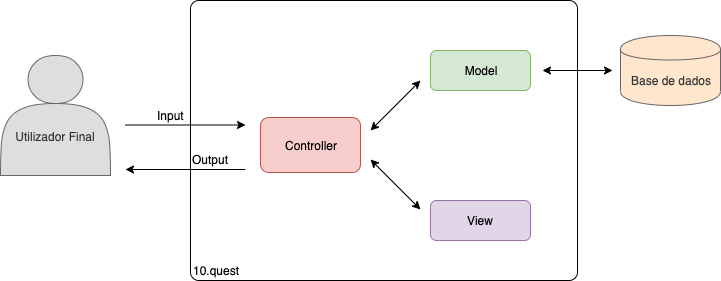
\includegraphics[width=1\textwidth]{img/arq/diagrama-MVC}
		\caption{Estrutura do Sistema}
		\label{fig:arq-mvc}
	\end{center}
\end{figure}

O componente \textbf{Model} controla a organização e armazenamento dos dados. Este módulo representa os dados que são transferidos entre os componentes Controller e View mas não representa nenhuma lógica no que diz respeito ao que é representado na camada de apresentação.

O componente \textbf{View} pode ser considerada a camada de apresentação. Este componente contém todas os ingredientes que constituem as interfaces do utilizador e controla a forma como a informação lhe é apresentada. Este modelo sabe como aceder ao modelo de dados que é apresentado ao utilizador contudo não sabe como o manipular nem o que significa.

Por último temos o componente \textbf{Controller}.  Este componente atua entre os modelos View e Model reagindo a eventos na View e respondendo a estes pedidos manipulando os dados utilizando o componente Model e interagindo com o componente View para renderizar o \textit{output}.


\subsection{Modelo C4}

Nesta secção encontra-se representada e descrita toda a arquitetura da plataforma 10.quest,  influenciada pelos objetivos de negócio, \textit{stakeholders}, requisitos e restrições técnica e de negócio, apresentados anteriormente.

Foram utilizados três diagramas para representar a arquitetura do sistema, utilizando o \textbf{modelo C4}\cite{c4}: diagrama de contexto, diagrama de contentores e o diagrama de componentes.

Os diferentes diagramas representam diferentes perspetivas e níveis de abstração e foram feitos com o intuito de facilitar a compreensão da arquitetura permitindo à equipa de desenvolvimento visualizar os diferentes níveis de granularidade. 

O diagrama de contexto mostra a relação entre o sistema que vai ser desenvolvido e outros agentes como, por exemplo, utilizadores e sistemas externos.  Este é o diagrama com maior nível de abstração e é bom para sublinhar as dependências externas que a equipa de desenvolvimento tem que integrar no sistema. 

O diagrama de contentores apresenta um maior detalhe (i. e. relativamente ao diagrama de contexto) e mostra os diferentes contentores que constituem o sistema (e. g. bases de dados, aplicações, microserviços etc...). Neste diagrama são também definidas algumas decisões arquiteturais. 

Por último temos o diagrama de componentes que aproxima um contentor individualmente e mostra todos os componentes que constituem esse contentor. Desta forma conseguimos perceber as principais funcionalidades do sistema. 


\subsubsection{Diagrama de Contexto}

Como foi referido no Capítulo \ref{sec:introducao} o 10.quest é uma plataforma de inbound marketing que consiste num \textit{backoffice} para criação de questionários, concursos e criação de formulário com o auxílio do \acrshort{tcg}.

Como podemos ver na Figura \ref{fig:arq-contexto} o 10.quest interage com seis sistemas externos. O SendGrid\cite{sg} é um \acrshort{saas}, na \textit{cloud}, que fornece um serviço de entrega de emails. Este serviço permite enviar emails através de APIs flexíveis garantindo uma disponibilidade  de 99.999\% \cite{sguptime}. 
O TCG, tal como foi referido no Capítulo \ref{sec:estado-arte}, é uma plataforma de criação de formações que tem como principal objectivo, transmitir conhecimento através de uma técnica de aprendizagem baseada em tentativa e erro Algumas das funcionalidades do \acrshort{tcg} serão utilizadas pelo 10.quest.
Para partilhar os questionários, concursos e formações o 10.quest irá utilizar as APIs do Facebook, LinkedIn, Twitter e Instagram.


\newpage

\begin{figure}[ht!]
	\begin{center}
		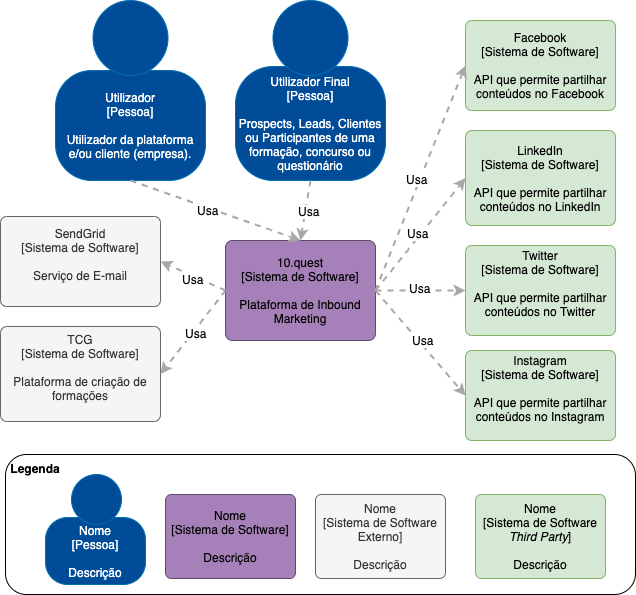
\includegraphics[width=0.9\textwidth]{img/arq/diagrama-contexto}
		\caption{Diagrama de Contexto}
		\label{fig:arq-contexto}
	\end{center}
\end{figure}

\subsubsection{Diagrama de Contentores}

Na Figura \ref{fig:arq-contentores} está representado o diagrama de contentores, onde se pode observar com mais detalhe a constituição do sistema de software.

Os utilizadores podem ser de dois tipos: o utilizador do backoffice que tem acesso a todas as funcionalidade da plataforma e o utilizador final que tem acesso a uma página web para participar nas formações, concursos e ou questionários.

A aplicação web efetua os pedidos dos utilizadores, através de pedidos \acrshort{https}/\acrshort{rest} à API. A aplicação web será a camada de apresentação da API e ambos serão desenvolvidos em Django. A API será o contentor responsável por tratar de todos os pedidos efetuados pelos utilizadores do \textit{backoffice}. Para este efeito a API implementa um conjunto de funcionalidades, representadas na Figura \ref{fig:arq-componentes1}, que manipulam um conjunto de dados armazenados numa base de dados relacional PostgreSQL, para conseguir as informações necessárias.
\newpage

\begin{figure}[ht!]
	\begin{center}
		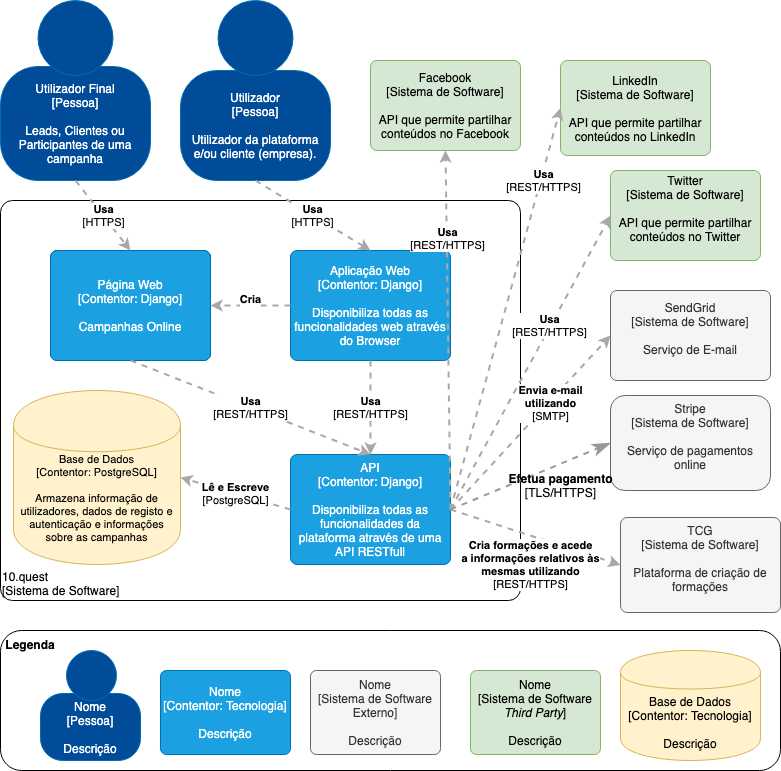
\includegraphics[width=0.9\textwidth]{img/arq/diagrama-contentores}
		\caption{Diagrama de Contentores}
		\label{fig:arq-contentores}
	\end{center}
\end{figure}

\subsubsection{Diagrama de Componentes}

Na Figura \ref{fig:arq-componentes} é apresentado o diagrama de componentes e na Figura \ref{fig:arq-componentes1} são apresentados os componentes da API. 

A autenticação é necessária para que os pedidos sejam aceites e mapeados pela API. Para isto a componente "Autenticação", permite ao utilizador efetuar a sua autenticação e verifica a autenticidade do mesmo, em cada pedido, através de tokens. Desta forma, caso o utilizador esteja autenticado os seus pedidos \acrshort{https}/\acrshort{rest} avançam para a componente API , que inclui todas as componente (i. e. funcionalidades) que dão resposta aos requisitos funcionais definidos para o projeto.

A componente "Dados" permite às restantes componentes interagir com a base de dados, tanto para ler, como para escrever.


\begin{figure}[ht!]
	\begin{center}
		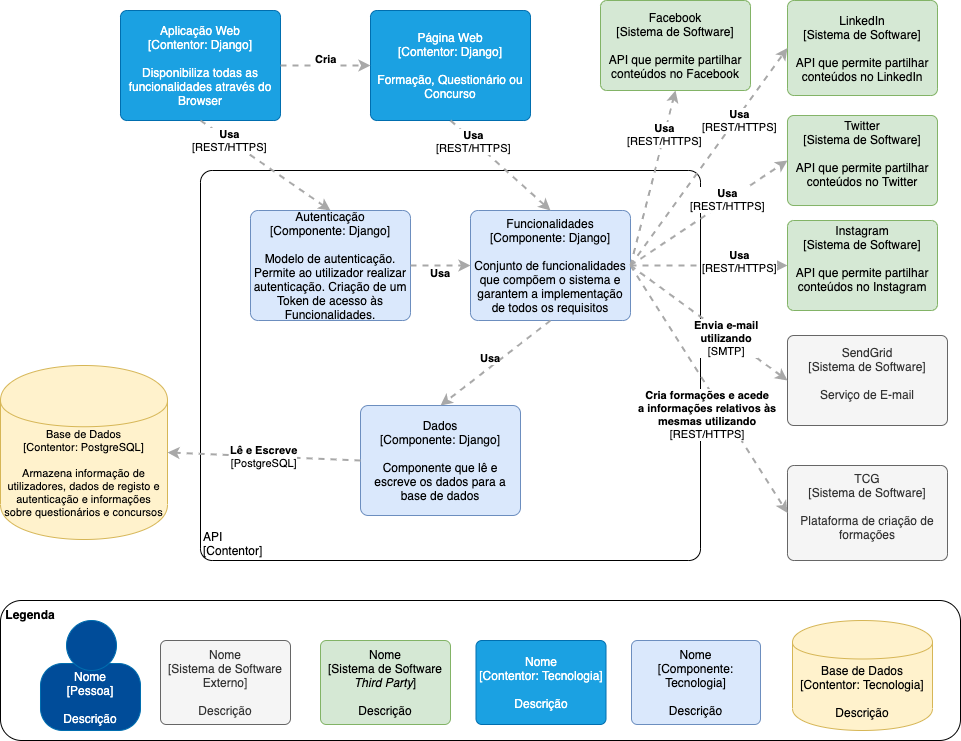
\includegraphics[width=0.86\textwidth]{img/arq/diagrama-componentes}
		\caption{Diagrama de Componentes}
		\label{fig:arq-componentes}
	\end{center}
\end{figure}

\begin{figure}[ht!]
	\begin{center}
		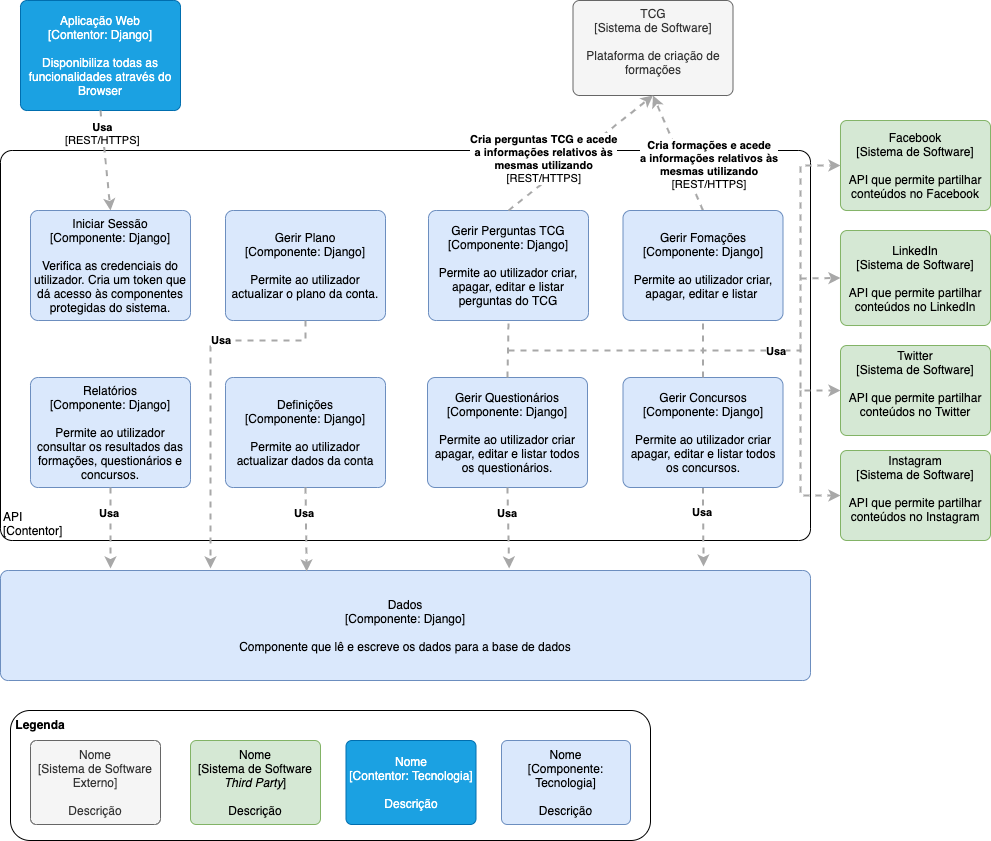
\includegraphics[width=0.87\textwidth]{img/arq/diagrama-componentes1}
		\caption{Diagrama Componentes da componente Funcionalidades}
		\label{fig:arq-componentes1}
	\end{center}
\end{figure}

\newpage


\subsection{Diagrama Entidade Relacionamento}

Nesta secção é apresentado o diagrama conceitual que representa a base de dados do projecto desenvolvido. De seguida é dada uma breve descrição de todas as classes presentes na Figura \ref{fig:arq-er}. 

\begin{figure}[ht!]
	\begin{center}
		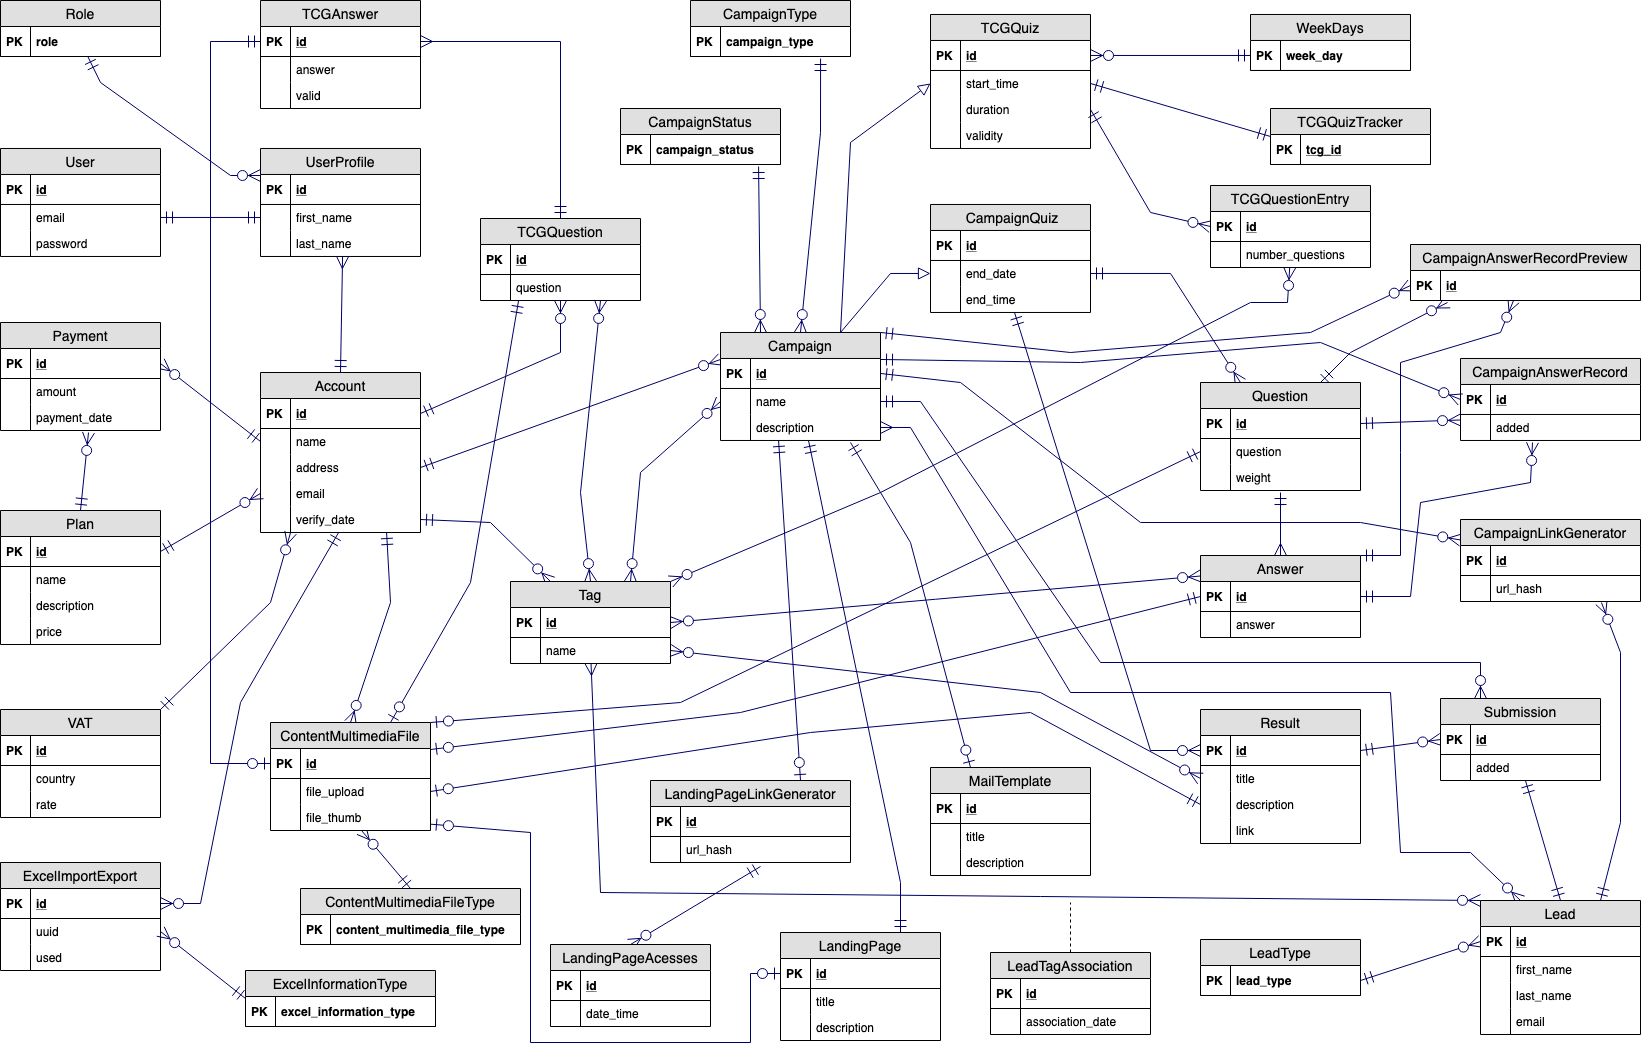
\includegraphics[width=0.87\textwidth]{img/arq/er}
		\caption{Diagrama Entidade Relacionamento - Modelo Conceitual}
		\label{fig:arq-er}
	\end{center}
\end{figure}

Com este diagrama, represetado na Figura \ref{fig:arq-er} conseguimos perceber são as entidades e como se relacionam entre si dentro do sistema.

\begin{itemize}
	\item[--] \textbf{CampaignAnswerRecordPreview}: 
		\subitem \underline{}
		\subitem \underline{}
	\item[--] \textbf{CampaignAnswerRecord}: 
		\subitem \underline{}
		\subitem \underline{}
	\item[--] \textbf{CampaignLinkGenerator}: 
		\subitem \underline{}
		\subitem \underline{}
	\item[--] \textbf{Submission}: 
		\subitem \underline{}
		\subitem \underline{}
	\item[--] \textbf{Lead}: Esta entidade representa a informação associada às \textit{leads}. Está directamente relacionada com:
		\subitem \underline{Campaign}: Uma lead partipica em uma ou mais campanhas.
		\subitem \underline{Tag}: Uma lead têm multiplas tags associadas para traçar um pefil de personalidade.
	\item[--] \textbf{MailTemplate}: Esta entidade representa a informação que é enviada no mail para os participantes das campanhas. Está directamente relacionada com:
		\subitem \underline{Campaign}: Um \textit{template} de mail representa informação associada a uma campanha.
	\item[--] \textbf{ExcelImportExport}: Esta entidade controla o carregamento de ficheiros excel na plataforma para garantir a integridade dos dados. Está directamente relacionada com:
		\subitem \underline{Account}: Um registo desta entidade está associada a uma conta de empresa.
		\subitem \underline{ExcelInformationType}: O tipo de ficheiro excel identifica o tipo de informação que é carregado.
	\item[--] \textbf{ExcelInformationType}: Esta entidade representa o tipo do ficheiro excel. Os ficheiros excel podem ser do tipo: perguntas de questionários de personalidade, resultados de questionários de personalidade ou perguntas de formação.
	\item[--] \textbf{UserProfile}: Esta entidade representa a conta de um utilizador da plataforma. Está diretamente relacionada com:
		\subitem \underline{User}: Esta conta está associada a uma entidade que guarda os dados de registo e permissões do utilizador.
		\subitem \underline{Account}: Esta conta está associada a uma conta de empresa.
		\subitem \underline{Role}: Esta conta tem uma função sobre a conta da empresa que pode ser de administrador ou colaborador. Dependendo da função têm permissões diferentes.
	\item[--] \textbf{Account}: Esta entidade representa a conta da empresa, da plataforma. Está diretamente relacionada com:
		\subitem \underline{Plan}: Uma conta subscreve um plano.
		\subitem \underline{VAT}: Uma conta sofre o imposto do respectivo país.
	\item[--] \textbf{LeadTagAssociation}: Esta entidade guarda a data em que uma determinada tag foi associada a uma \textit{lead}. Está directamente relacionada com:
		\subitem \underline{Tag}
		\subitem \underline{Lead}
	\item[--] \textbf{Result}: Esta entidade representa um resultado de um questionário de personalidade. Está directamente relacionado com:
		\subitem \underline{TCGQuiz}: Um resultado está associado a um questionário de personalidade.
		\subitem \underline{ContentMultimediaFile}: Um resultado pode ter uma imagem ou vídeo.
		\subitem \underline{Tag}: Um resultado pode ter multiplas tags, que vão ser associadas a um participante (i.e. \textit{lead}) caso saia ao mesmo.
	\item[--] \textbf{TCGAnswer}: Esta entidade representa uma resposta a uma pergunta de uma formação. Está directamente relacionado com:
		\subitem \underline{TCGQuestion}: Uma resposta pertence a uma pergunta.
		\subitem \underline{ContentMultimediaFile}: Uma resposta pode ter uma imagem ou vídeo.
	\item[--] \textbf{Answer}: Esta entidade representa uma resposta a uma pergunta de um questionário de personalidade. Está directamente relacionado com:
		\subitem \underline{Question}: Uma resposta pertence a uma pergunta.
		\subitem \underline{ContentMultimediaFile}: Uma resposta pode ter uma imagem ou vídeo.
	\item[--] \textbf{TCGQuetionEntry}: Esta entidade representa uma entrada de perguntas de formação. Está directamente relacinada com:
		\subitem \underline{TCGQuiz}: Uma entrada tem uma formação associada.
		\subitem \underline{Tag}: Uma entrada tem uma ou mais tags associadas. As tags representam as perguntas associadas à entrada (i.e as perguntas com as tags correspondentes).
	\item[--] \textbf{TCGQuestion}: Esta entidade representa uma pergunta de uma formação. Está diretamente associado com:
		\subitem \underline{Account}: Uma pergunta de uma formação está associada a uma conta de empresa.
		\subitem \underline{Tag}: Uma pergunta pode ter multimas tags associadas.
		\subitem \underline{ContentMultimediaFile}: Uma pergunta pode ter uma imagem ou video associado.
	\item[--] \textbf{Question}: Esta entidade representa uma pergunta de um questionário de personalidade. Está diretamente associado com:
		\subitem \underline{CampaignQuiz}: Uma pergunta percente a uma questionário de personalidade.
		\subitem \underline{Answer}: Uma pergunta tem entre 2 a 4 respostas.
		\subitem \underline{ContentMultimediaFile}: Uma pergunta pode ter uma imagem ou vídeo.
		\subitem \underline{CampaignAnswerRecord}: Registo de resposta a uma pergunta.
		\subitem \underline{CampaignAnswerRecordPreview}: Registo de resposta a uma pergunta em modo de visualização.
	\item[--] \textbf{LandingPageAcesses}: Esta entidade guada o registo de acessos à página de apresentação. Está diretamente relacionado com:
		\subitem \underline{LandingPageLinkGenerator}: Um acesso é feito através do acesso ao link da página de apresentação.
	\item[--] \textbf{LandingPageLinkGenerator}: Esta entidade representa o link da pagina de apresentação. 
	\item[--] \textbf{LandingPage}: Esta entidade representa a página de apresentação da campanha. Está diretamente relacionada com:
		\subitem \underline{Campaign}: Uma pagina de apresentação, apresenta uma campanha.
		\subitem \underline{ContentMultimediaFile}: Uma pagina de apresentação pode ter uma imagem ou vídeo.
	\item[--] \textbf{Payment}: Esta entidade representa o registo de todos os pagamentos efectuados. Está diretamente relacionada com:
		\subitem \underline{Account}: O Pagamento é efectuado por uma determinada conta.
		\subitem \underline{Plan}: O Pagamento corresponde a um determinado plano.
	\item[--] \textbf{TCGQuizTracker}: Esta entidade guarda o identificador da campanha, da base de dados do The CompanyGym.
	\item[--] \textbf{Campaign}: Esta entidade representa uma campanha.  Está diretamente relacionada com:
		\subitem \underline{Tag}: Uma campanha pode ter multiplas tags associadas.
		\subitem \underline{Account}: Uma campanha está associada a uma conta de empresa.
		\subitem \underline{LandingPage}: Uma campanha tem uma \textit{Landing Page}.
		\subitem \underline{LandingPageLinkGenerator}: Link de acesso à respectiva \textit{Landing Page}. 
		\subitem \underline{MailTemplate}: Uma campanha pode ter um template personalizado de mail.
		\subitem \underline{Lead}: Os participantes de uma campanha tornam-se \textit{leads}.
		\subitem \underline{CampaignLinkGenerator}: Uma campanha tem um link.
		\subitem \underline{Submission}: Uma submissão tem uma campanha associada.
		\subitem \underline{CampaignAnswerRecord}: Um registo de uma resposta a uma pergunta tem uma campanha associada.
		\subitem \underline{CampaignAnswerRecordPreview}: Um registo de uma resposta a uma pergunta, em modo de visualização, tem uma campanha associada.
		\subitem \underline{CampaignType}: Uma campanha pode ser do tipo: concurso, questionário de personalidade ou formação.
		\subitem \underline{CampaignStatus}: Uma campanha passa por várias estados: rascunho, completa, online e terminada.
	\item[--] \textbf{Plan}: Esta entidade representa os planos da plataforma. Está diretamente relacionado com:
		\subitem \underline{Account}: Uma conta subscreve um plano.
		\subitem \underline{Payment}: Um pagamento têm um plano associado.
	\item[--] \textbf{Tag}: Esta entidade representa uma tag. Estas tags são associadas a outras entidades para traçar caracteristicas da mesma:
		\subitem \underline{Account}: Uma tag está associada a uma conta de empresa.
		\subitem \underline{Campaign}: Uma campanha pode ter multiplas tags que serão associadas mais tarde aos participantes da mesma.
		\subitem \underline{Result}: Um resultado pode ter multiplas tags que serão associadas aos participantes a quem saia o mesmo.
		\subitem \underline{TCGQuestion}: Uma pergunta de uma formação pode ter multiplas tags associadas.
		\subitem \underline{TCGQuestionEntry}: Uma entrada de perguntas de formação, pode ter multiplas tags que representam as perguntas que têm essas mesmas tags associadas.
		\subitem \underline{Answer}: Um resultado pode ter multiplas tags associadas. As tags das respostas são associadas aos participantes (i.e.\textit{leads}) dos questionários de personalidade e utilizadas para calcular o resultado final.
		\subitem \underline{Lead}: Uma \textit{lead} pode ter multiplas tags associadas que permite traçar perfis de personalidade.
	\item[--] \textbf{VAT}: VAT (\textit{Value Added Tax}) representa o imposto correspondente a cada país.
	\item[--] \textbf{ContentMultimediaFile}: Esta entidade representa o conteudo multimédia carregador pelos utilizadores na plataforma. Está diretamente relacionado com:
		\subitem \underline{Account}: Um conteúdo multimédia está associado a uma conta de empresa.
		\subitem \underline{ContentMultimediaFileType}: Um conteúdo multimédia por ser uma imagem ou um vídeo.
	\item[--] \textbf{ContentMultimediaFileType}: Esta entidade representa o tipo de ficheiro multimédia. Estes tipos podem ser:  Imagem ou Video.
	\item[--] \textbf{CampainStatus}: Esta entidade representa o estado das campanhas. Estes estados podem ser: Rascunho, Completo, Online e Terminado.
	\item[--] \textbf{Role}: Esta entidade representa o tipo de função de um utilizador da plataforma. Estas funções podem ser Administrador ou Colaborador.
	\item[--] \textbf{LeadType}: Esta entidade representa o tipo de \textit{Lead}. Nem sempre os participantes terminam a participação nas campanhas e portanto uma \textit{Lead} pode ser do tipo: Qualificada ou Não Qualificada.
	\item[--] \textbf{CampaignType}: Esta entidade representa o tipo da campanha. As campanhas podem ser do tipo: Questionários de Personalidade, Concursos ou Formações. 
	\item[--] \textbf{WeekDays}: Esta entidade representa o dia da semana. A tabela na base de dados apenas tem 7 entradas, uma para cada dia da semana.
\end{itemize}

%  FALTA CAPITULO PARA DISCUSSÂO VALIDAÇÂO DA ARQUITECTURA. Escrever assim que todas as decisões estiveres feitas

\subsection{Tecnologias Utilizadas}

Grande parte das tecnologias ainda estão por definir. 

\section{Análise de Riscos}
\label{analiseriscos}

Antes de se inicializar a fase de desenvolvimento do projeto é importante realizar uma análise aos possíveis riscos associados ao projeto. Desta forma é importante antecipar/identificar os diferentes riscos que contribuem para o insucesso do projeto para que se possam criar estratégias de mitigação de maneira a minimizar o impacto de cada risco. Os diferentes riscos serão classificados tendo em conta o seu impacto e a sua probabilidade.

\begin{itemize}
	\item[--] \textbf{Probabilidade}
		\subitem \textbf{Baixa}: Menor que 30\%
		\subitem \textbf{Média}: Entre 30\% a 70\%
		\subitem \textbf{Alta}: Superior a 70\%
	\item[--] \textbf{Impacto}
		\subitem \textbf{Baixo}: Interfere no desenvolvimento do projecto.
		\subitem \textbf{Médio}: Interfere no desenvolvimento do projecto e força alterações no produto final.
		\subitem \textbf{Alto}: Compromete a finalização do projeto.
\end{itemize}

De seguida serão listados todos os riscos associados ao projeto e respectivo plano de mitigação para tentar reduzir o impacto do mesmo:

\textbf{R01 - Dependência de sistemas externos}
\begin{itemize}
	\item[--] \textbf{ID}: R01
	\item[--] \textbf{Descrição}: Não se pode garantir uma disponibilidade de 100\% em todos os sistemas externos (e. g. APIs offline) sendo que em algumas ocasiões o sistema pode ter algumas funcionalidades indisponíveis.
	\item[--] \textbf{Estratégia de Mitigação}: Quando um serviço externo está temporariamente indisponível, apesar algumas funcionalidades também indisponíveis, o sistema deve tratar os pedidos do utilizador de forma a afetar a experiência do utilizador, ou no pior dos casos para reduzir o impacto no mesmo.
	\item[--] \textbf{Probabilidade}: Baixa
	\item[--] \textbf{Impacto}: Baixo
\end{itemize}

\textbf{R02 - Dificuldade em implementar o sistema de pagamento}
\begin{itemize}
	\item[--] \textbf{ID}: R02
	\item[--] \textbf{Descrição}: A falta de experiência por parte do aluno na implementação de métodos ou serviços de pagamentos põe em causa a boa implementação do mesmo e pode comprometer uma das principais funcionalidades do produto final.
	\item[--] \textbf{Estratégia de Mitigação}: Deve ser feita uma análise cuidada dos métodos ou serviços de pagamentos disponíveis para integrar com a tecnologia de desenvolvimento da plataforma e de seguida deve ser lida a documentação com atenção para garantir uma boa implementação da mesma.
	\item[--] \textbf{Probabilidade}: Alta
	\item[--] \textbf{Impacto}: Alto
\end{itemize}

\textbf{R03 - Adaptação a novas tecnologias }
\begin{itemize}
	\item[--] \textbf{ID}: R03
	\item[--] \textbf{Descrição}: A não familiarização, por parte do aluno, com as principais tecnologias que irão ser utilizadas na desenvolvimento do projeto, pode criar atrasos implementação devido à falta de experiência e/ou subestimação do tempo definido para cada tarefa, comprometendo a implementação de algumas funcionalidades.
	\item[--] \textbf{Estratégia de Mitigação}: Para além das horas definidas no planeamento do projeto, o aluno terá de dispensar horas extra de modo a conseguir concluir a implementação e validação de todas as funcionalidades.
	\item[--] \textbf{Probabilidade}: Média
	\item[--] \textbf{Impacto}: Médio
\end{itemize}

\textbf{R04 - Novo requisito funcional}
\begin{itemize}
	\item[--] \textbf{ID}: R04
	\item[--] \textbf{Descrição}: As necessidades do cliente podem mudar com o tempo e nesse sentido é possível o aparecimento de um novo requisito funcional.
	\item[--] \textbf{Estratégia de Mitigação}: Reavaliação do plano de desenvolvimento e reestruturação de algumas funcionalidades para que fiquem mais genéricas e assim possa haver tempo para a realização do(s) novo(s) requisito(s). Em alternativa poderão também ter que ser dispensadas algumas horas pelo aluno de modo a cumprir com o plano de desenvolvimento.
	\item[--] \textbf{Probabilidade}: Baixa 
	\item[--] \textbf{Impacto}: Médio
\end{itemize}

Para uma melhor compreensão e visualização dos riscos associados ao projecto será apresentado de seguida, na Tabela \ref{tab:riscos}, um resumo da probabilidade e o impacto de cada risco.

\pagebreak
\mbox{}
\begin{table}
	\centering
\begin{tabular}{ | l | l | l | l |}
	\hline
	\diagbox[width=15em]{Impacto}{Probabilidade}
	& Baixo & Médio & Alto\\
	\hline
	Baixa & \cellcolor{green}\centering R01 & \cellcolor{yellow}R04& \cellcolor{orange}\\
	\hline
	Média & \cellcolor{yellow} & \cellcolor{orange}R03 & \cellcolor{darkOrange}\\
	\hline
	Alta & \cellcolor{orange} & \cellcolor{darkOrange} & \cellcolor{red}R02\\
	\hline
\end{tabular}
\begin{center}
\caption {Classificação dos riscos associados ao projecto}
\label {tab:riscos}
\end{center}
\end{table}



% Listar os Riscos em que activei a estratégia de mitigação e de seguida voltar a mostrar a tabela actualizada







%-------------------------------------------------------------------------------------------------
\blankpage
%-------------------------------------------------------------------------------------------------

\glsresetall
